\documentclass[12pt,a4]{article}




\usepackage{graphicx,amsmath,amssymb,amsthm, boxedminipage,xcolor}

%\usepackage[lined,boxed]{algorithm2e}

\usepackage{algorithm}
\usepackage{algpseudocode}

%\usepackage{algorithmic}
\usepackage{algpseudocode}
\usepackage{amsmath}
\usepackage{graphics}
\usepackage{epsfig}

\newtheorem{theorem}{Theorem}[section]
\newtheorem{proposition}[theorem]{Proposition}
\newtheorem{lemma}[theorem]{Lemma}
\newtheorem{corollary}[theorem]{Corollary}
\newtheorem{definition}[theorem]{Definition}

\newtheorem*{theorem*}{Theorem}
\newtheorem*{lemma*}{Lemma}
\newtheorem*{proposition*}{Proposition}


\newtheorem{exercise}[theorem]{Exercise}
\newtheorem{exerciseD}[theorem]{*Exercise}
\newtheorem{exerciseDD}[theorem]{**Exercise}

\let\oldexercise\exercise
\renewcommand{\exercise}{\oldexercise\normalfont}

%\let\oldexerciseD\exerciseD
%\renewcommand{\exerciseD}{\oldexerciseD\normalfont}

%\let\oldexerciseDD\exerciseDD
%\renewcommand{\exerciseDD}{\oldexerciseDD\normalfont}

\newcommand{\E}{\mathbb{E}}
%\newcommand{\nth}[1]{#1^{\textsuperscript{th}}}
\newcommand{\scalar}[2]{\ensuremath{\langle #1, #2\rangle}}
\newcommand{\floor}[1]{\left\lfloor #1 \right\rfloor}
\newcommand{\ceil}[1]{\left\lceil #1 \right\rceil}
\newcommand{\norm}[1]{\|#1\|}
\newcommand{\pfrac}[2]{\left(\frac{#1}{#2}\right)}
\newcommand{\nth}[1]{#1^{\textsuperscript{th}}}
\newcommand{\core}{\textnormal{core}}



\newif\ifsolution

\solutionfalse

\newcommand{\answer}[1]{
\ifsolution
{\color{blue} #1}
\else
\fi
}



\newcommand{\poly}{\textnormal{poly}}
\newcommand{\quasipol}{\textnormal{quasipol}}
\newcommand{\ssubexp}{\textnormal{stronglySubExp}}
\newcommand{\wsubexp}{\textnormal{weaklySubExp}}
\newcommand{\simplyexp}{\textnormal{E}}
\newcommand{\expo}{\textnormal{Exp}}



\newcommand{\N}{\mathbb{N}}
\newcommand{\nn}{\mathbb{N}_0^n}
\newcommand{\R}{\mathbb{R}}
\newcommand{\Z}{\mathbb{Z}}


\definecolor{darkgreen}{rgb}{0,0.6,0}


\date{}

\title{
  Mathematical Foundations \\of \\Computer Science\\
  \vspace{3mm}
{\normalsize CS 499,	Shanghai Jiaotong University,  Dominik Scheder}
}

\begin{document}

\maketitle

%\begin{quotation}
%  You are welcome to discuss the exercises in the discussion
%  forum. Please take them serious. Doing the exercises is as important
%  than watching the videos.
%
%  I intentionally included very challenging exercises and marked them
%  with one or two ``$*$''. No star means you should be able to solve
%  the exercises without big problems once you have understood
%  the material from the video lecture. One star means it requires 
%  significant additional thinking. Two stars means it is not 
%  unlikely that you will fail to solve them, even once you have understood
%  the material and thought a lot about the exercise. Don't feel bad
%  if you fail. Failure is part of learning.
%
%  This is the first time this course is online. Thus there might be mistakes
%  (typos or more serious conceptual mistakes) in the exercises. I will be 
%  grateful if you point them out to me!
%\end{quotation}





\setcounter{section}{7}

\section{Spanning Trees}



\begin{itemize}
 \item Homework assignment published on Monday, 2018-04-16
 \item Submit questions and first solution by Sunday, 2018-04-22, 12:00, by email to me and the TAs.
 \item Submit your final solution by Sunday, 2018-04-29.
\end{itemize}

\subsection{Minimum Spanning Trees}





Throughout this assignment, let $G = (V,E)$ be a connected graph
and $w: E \rightarrow \R^+$ be a weight function.\\

\begin{exercise}
    Prove the inverse of the cut lemma:
      If $X$ is good, $e \not \in X$, and $X \cup e$ is good,
      then there is a cut $S, V\setminus S$ such that (i) no
      edge from $X$ crosses this cut and (ii) $e$ is a minimum
      weight edge of $G$ crossing this cut.
\end{exercise}
\begin{proof}
    Since $X \cup \{e\}$ is good, let $\{e\}\in T$, and $T$ and a minimum spanning tree. Delete $e$ in $T$ and then we will get two connected components. Let $S$ be the set of vertices in one connected component.

    (i) Because obviously $X\subset T$, and $e$ is the only element that crosses the cut, $X$ has no edge that crosses the cut.

    (ii) Assume there exists an edge $e'$ with a smaller weight than $e$. Because it is not chosen when forming the spanning tree, it must form a cycle in $S$ or $V\setminus S$. Otherwise, at that step of considering $e'$, $e$ has not been in the spanning tree, and then $e'$ cannot form a cycle across the cut.
\end{proof}

\begin{definition}
  For $c \in \R$ and a weighted graph $G = (V,E)$, let
  $G_c := (V, \{e \in E \ | \ w(e) \leq c\})$. That is, $G_c$ is the
  subgraph of $G$ consisting of all edges of weight at most $c$.
\end{definition}

\begin{lemma}
  Let $T$ be a minimum spanning tree of $G$, and let $c \in \R$.  Then
  $T_c$ and $G_c$ have exactly the same connected components.  (That
  is, two vertices $u,v \in V$ are connected in $T_c$ if and only if
  they are connected in $G_c$).
  \label{lemma-CC}
\end{lemma}

\begin{exercise}
     Illustrate Lemma~\ref{lemma-CC} with an example!
\end{exercise}

\textbf{Solution.}
\par 
$V=\{v_1,v_2\},E=\{(v_1,v_2)\}$, $T=\{(v_1,v_2)\}$. Obviously they are the same.

    

\begin{exercise}
     Prove the lemma.
\end{exercise}

\begin{proof}
    In \emph{Kruskal Algorithm}, $\forall c \in \R, \forall e_i$ that $w(e)\leq c$, at the step considering it, if we can put $e_k$ in $T$, then we can put it in $T_c$, which will result in $T_c$'s connected component reduced by one, and since it does not cause a cycle in $T_c$, it does not cause a cycle in $G_c$, which will reduce $G_c$'s connected components by one. If we cannot add it into $T$, obviously this edge does not affect $T_c$, and since it causes a cycle in $T$, it will not reduce the connected components when added to $G_c$. In conclusion, each edge has the same influence on $T_c$ and $G_c$ at the step selecting them.
\end{proof}

\begin{definition}
  For a weighted graph $G$, let $m_c(G) := | \{ e \in E(G) \ | \ w(e) \leq c\}|$, i.e.,
  the number of edges of weight at most $c$ (so $G_c$ has $m_c(G)$ edges).
\end{definition}

\begin{lemma}
  Let $T, T'$ be two minimum spanning trees of $G$. Then
  $m_c(T) = m_c(T')$.
  \label{lemma-weight-multiplicity}
\end{lemma}

\begin{exercise}
Illustrate Lemma~\ref{lemma-weight-multiplicity} with an example!
\end{exercise}

\textbf{Solution.}
\par
    $V=\{v_1,v_2\},E=\{(v_1,v_2)\}$, $T=\{(v_1,v_2)\}$. Obviously they are the same.


\begin{exercise}
Prove the lemma.
\end{exercise}
\begin{proof}
$$
    m_c(T)=m_{+\infty}(T_c)=|E|-\text{connected component}(T_c)=|E|-\text{connected component}(G_c)=|E|-\text{connected component}(T'_c)=m_{+\infty}(T'_c)=m_c(T')
$$
\end{proof}

\begin{exercise}
  Suppose no two edges of $G$ have the same weight.
  Show that $G$ has exactly one minimum spanning tree!
\end{exercise}

\begin{proof}
    Obviously it is true considering \emph{Kruskal Algorithm} since every step they make the same decision.
\end{proof}









\subsection{Counting Special Functions}



In the video lecture, we have seen a connection between functions $f: V \rightarrow V$
and trees on $V$. We used this to learn something about the number of such trees.
Here, we will go in the reverse direction: the connection will actually teach us a bit
about the number of functions with a special structure.\\

Let $V$ be a set of size $n$. We have learned that there are $n^n$ functions $f: V \rightarrow V$.
For such a function we can draw an ``arrow diagram" by simply drawing an arrow from
$x$ to $f(x)$ for every $V$. For example, let $V = \{0,\dots,7\}$ and $f(x) := x^2 \mod 8$.
The arrow diagram of $f$ looks as follows:
\begin{center}
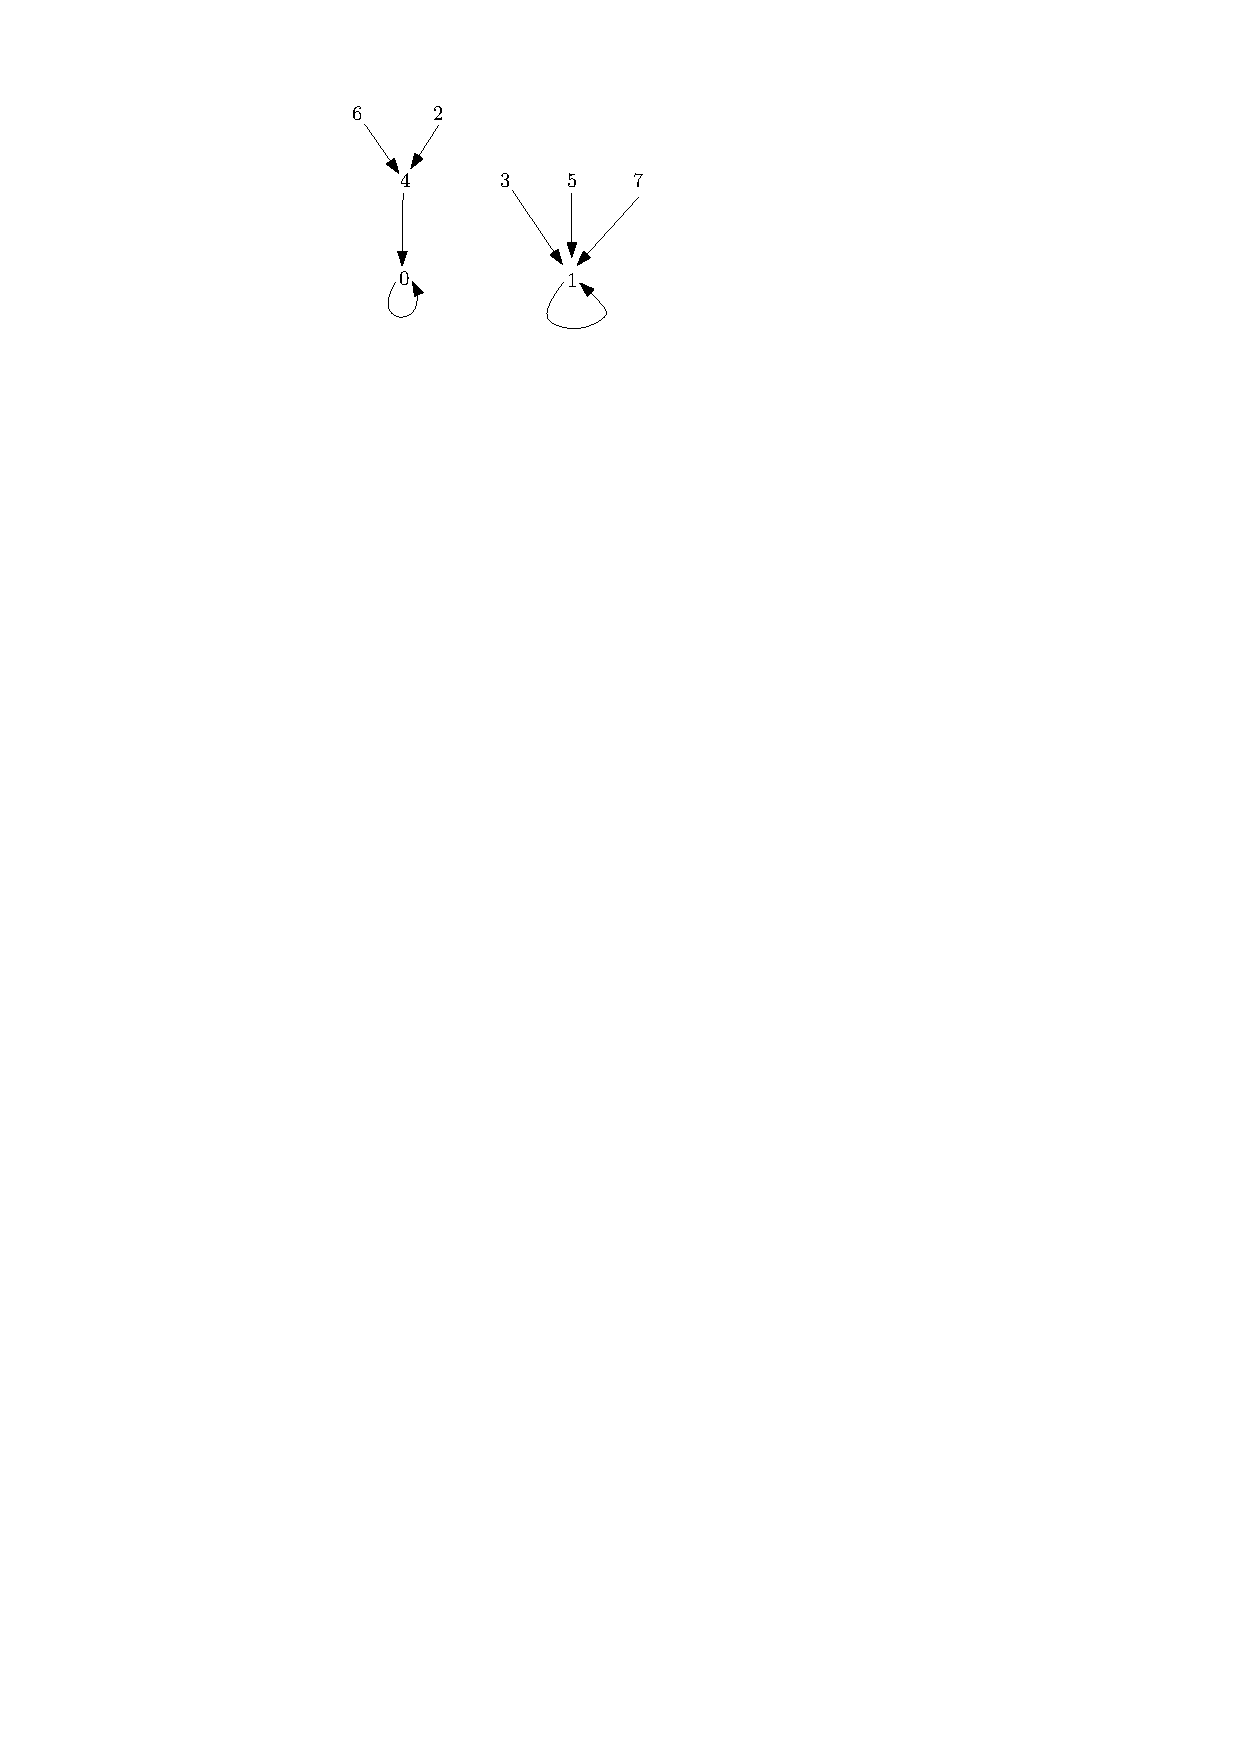
\includegraphics[width=0.3\textwidth]{figures/arrow-diagram.pdf}
\end{center}
The {\em core} of a function is the set of elements lying on cycles in such a diagram.
For example, the core of the above function is $\{0,1\}$. Formally, the core of $f$ is the
set
\begin{align*}
%\core(f) =
\{x \in V \ | \ \exists k \geq 1 f^{(k)}(x) = x \}
\end{align*}
where $f^{(k)}(x) = f( f( \dots f(x) \dots ))$, i.e., the function $f$ applied $k$ times
iteratively to $x$.

\begin{exercise}
Of the $n^n$ functions from $V$ to $V$, how many have a core of size $1$?
Give an explicit formula in terms of $n$.
\end{exercise}
\textbf{Solution.}
\par It is obvious that there are $n^{n-2}$ trees on $n$ vertices, with $n-1$ many edges. Because there is a function from $V$ to $V$, so there must be n edges in the graph. The one left forms a cycle and there are $n$ ways to choose the cycle because there are $n$ vertices. In total ,there are $n\times n^{n-2}= n^{n-1}$ functions.

\begin{exercise}
How many have a core of size $2$ that consists of two $1$-cycles? By this we mean
that $\core(f) = \{x,y\}$ with $f(x) = x$ and $f(y) = y$.
\end{exercise}
\textbf{Solution.}
\par This question is a little difficult because there is $n-2$ edges left regardless of the cycle. So let's divide the n vertices into $2$ parts(at least one vertex in a part) so there are $2^{n-1}-1$ ways to divide (because there is a symmetry). For each division, there are
\begin{equation*}
\tbinom{n}{2}
\end{equation*}
ways to choose the 2 left cycles. So the total number of functions is
\begin{equation*}
\tbinom{n}{2}\times (2^{n-1}-1)
\end{equation*}


\textbf{Hint.} For the previous two exercises, you need to use the link between functions
 $f: [n]\rightarrow [n]$ and
vertebrates $(T,h,b)$ from the video lecture.





\subsection{Counting Trees with Pr\"ufer Codes}

In the video lecture, we have seen Cayley's formula, stating that there are exactly
$n^{n-2}$ trees on the vertex set $[n]$. We showed a proof using
{\em vertebrates}. For this homework, read Section 7.4 of the textbook, titled
``A proof using the Pr\"ufer code''.


\begin{exercise}
  Let $V = \{1,\dots,9\}$ and consider the code $(1,3,3,2,6,6,1)$. Reconstruct a tree
  from this code. That is, find a tree on $V$ whose Pr\"ufer code is $(1,3,3,2,6,6,1)$.
\end{exercise}
\begin{center}
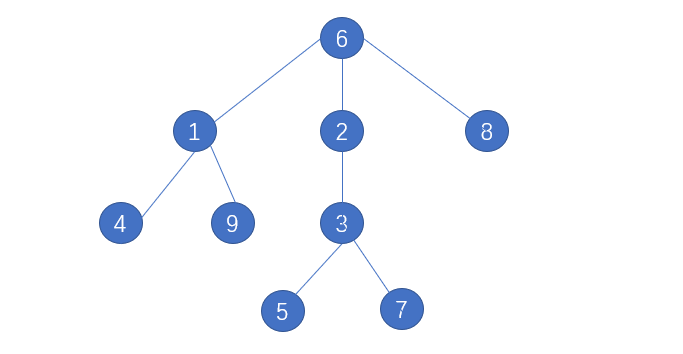
\includegraphics[width=0.3\textwidth]{./figures/prufer1.jpeg}
\end{center}
\begin{exercise}
  Let $\mathbf{p} = (p_1,p_2,\dots,p_{n-2})$ be the Pr\"ufer  code of some tree $T$ on $[n]$.
  Find a way to quickly determine the degree of vertex $i$ only by looking
  at $\mathbf{p}$ and not actually constructing the tree $T$.
  In particular, by looking at $\mathbf{p}$, what are the leaves of $T$?
\end{exercise}
\textbf{Solution.}
\par We assume the times vertex $i$ appear in the Pr\"ufer code is $i_t$, and it is obvious the degree of vertex is $i_t+1$ , and the the leaves of $T$ are the vertices which don't appear in the Pr\"ufer code.






\begin{exercise}
  Describe which tree on $V = [n]$  has the
  \begin{enumerate}
  \item Pr\"ufer code $(1,1,\dots,1)$.
  \item Pr\"ufer code $(1,2,3,\dots, n-2)$.
  \item Pr\"ufer code $(3,4,5,\dots, n)$.
  \item Pr\"ufer code $(n, n-1, n-2,\dots,4,3)$.
  \item Pr\"ufer code $(n-2,n-3,\dots,2,1)$.
  \item Pr\"ufer code $(1,2,1,2,\dots,1,2)$ (assuming $n$ is even).
 \end{enumerate}
 Justify and explain your answers.
\end{exercise}

\begin{figure}
\begin{center}
\caption{ }
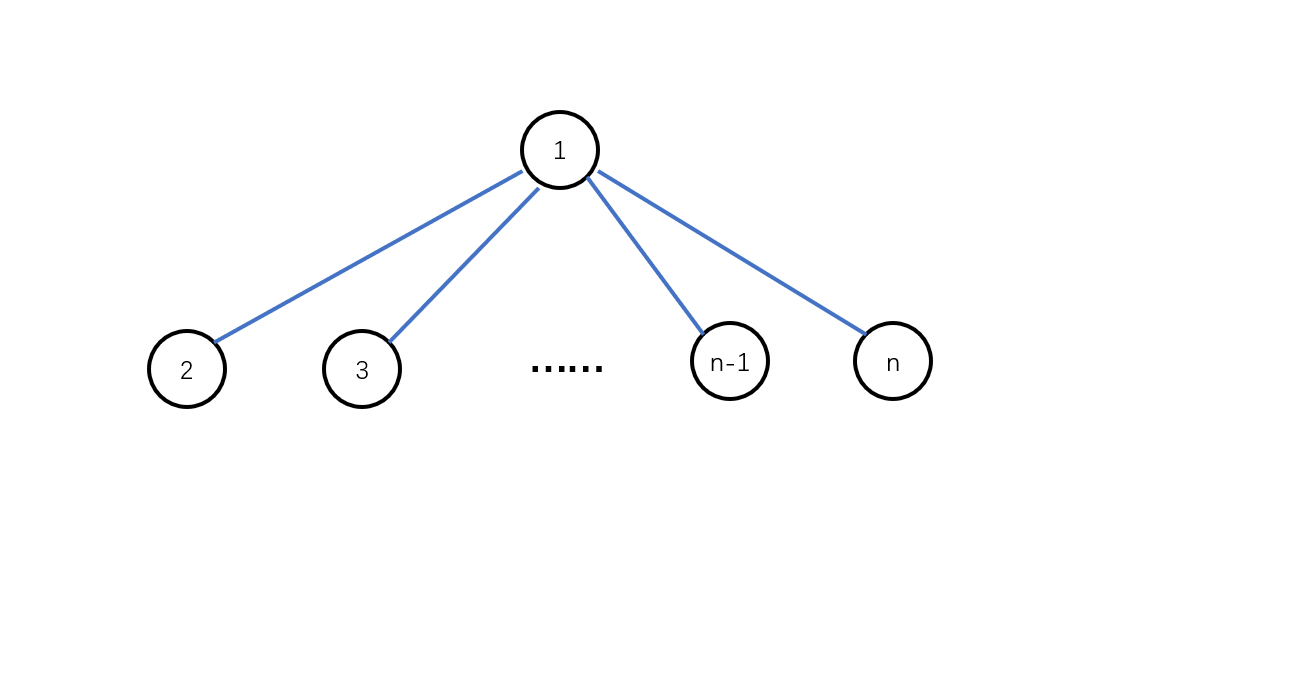
\includegraphics[scale=0.4]{figures/15_1.png}
\caption{ }
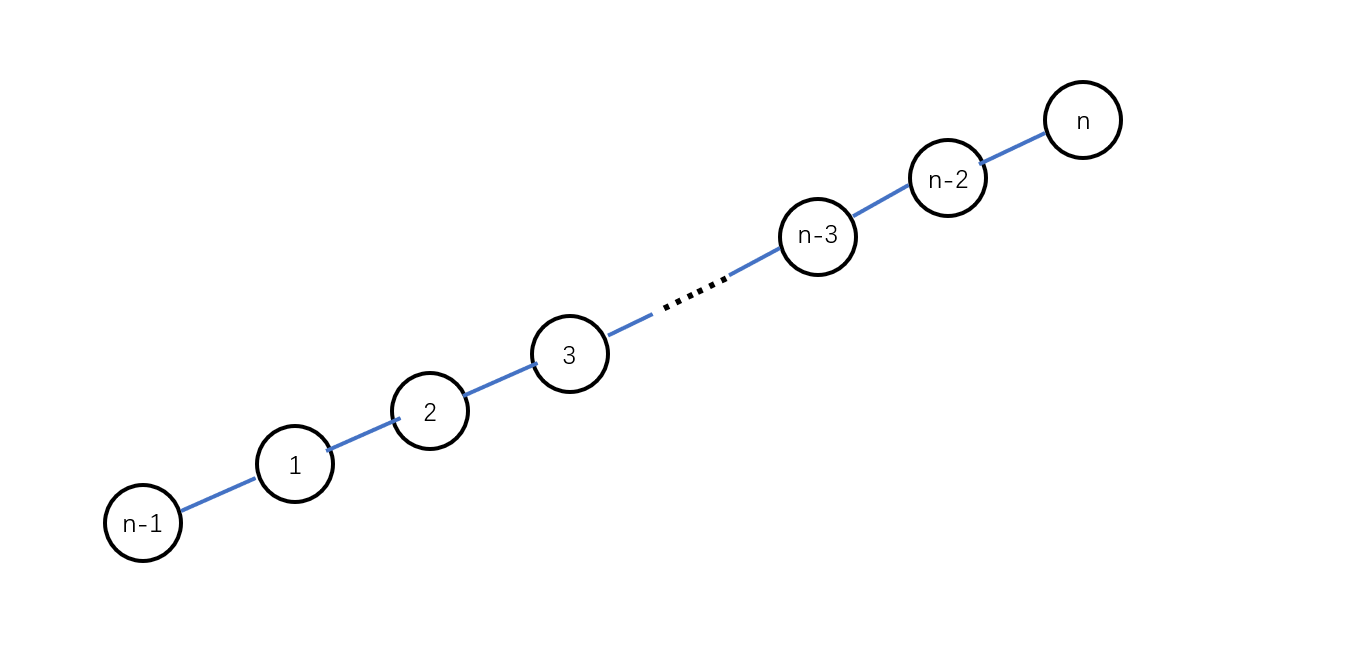
\includegraphics[scale=0.4]{figures/15_2.png}
\caption{ }
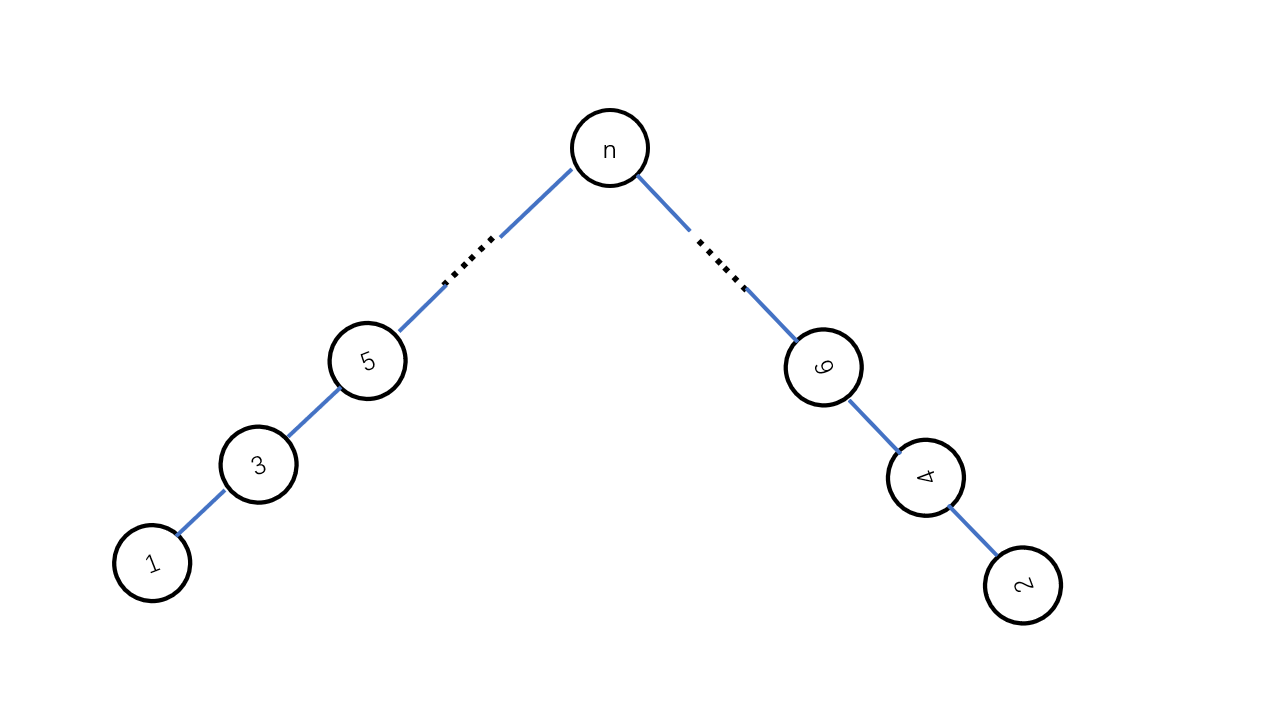
\includegraphics[scale=0.4]{figures/15_3.png}
\end{center}
\end{figure}
\begin{figure}
\begin{center}
\caption{ }
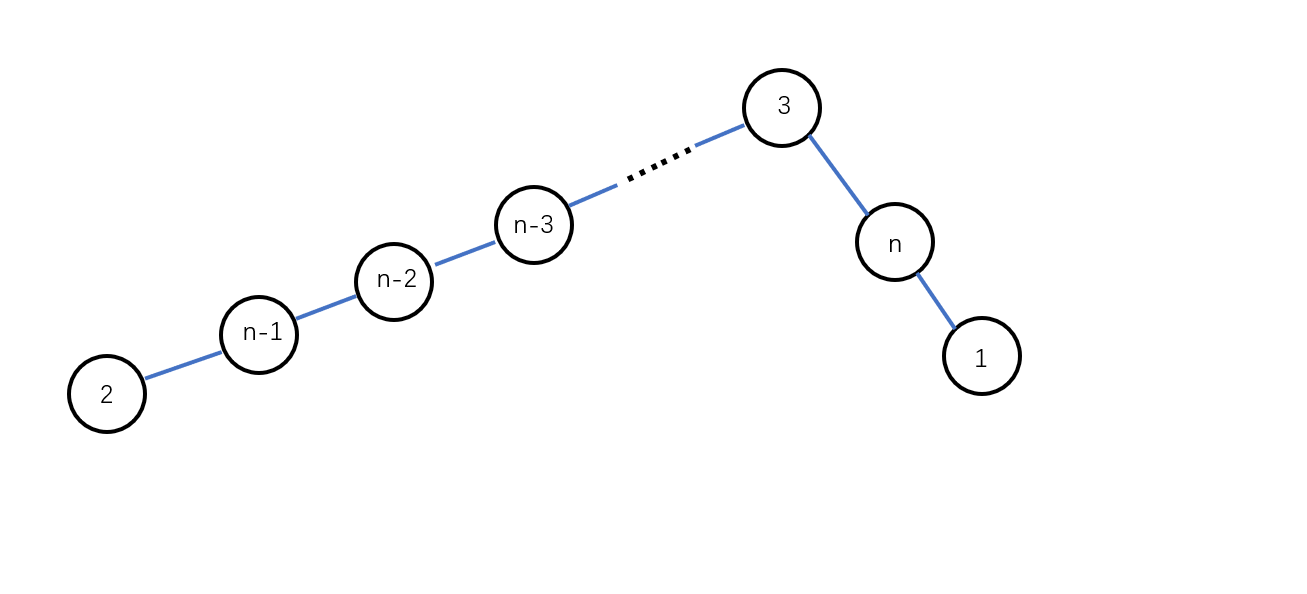
\includegraphics[scale=0.4]{figures/15_4.png}
\caption{ }
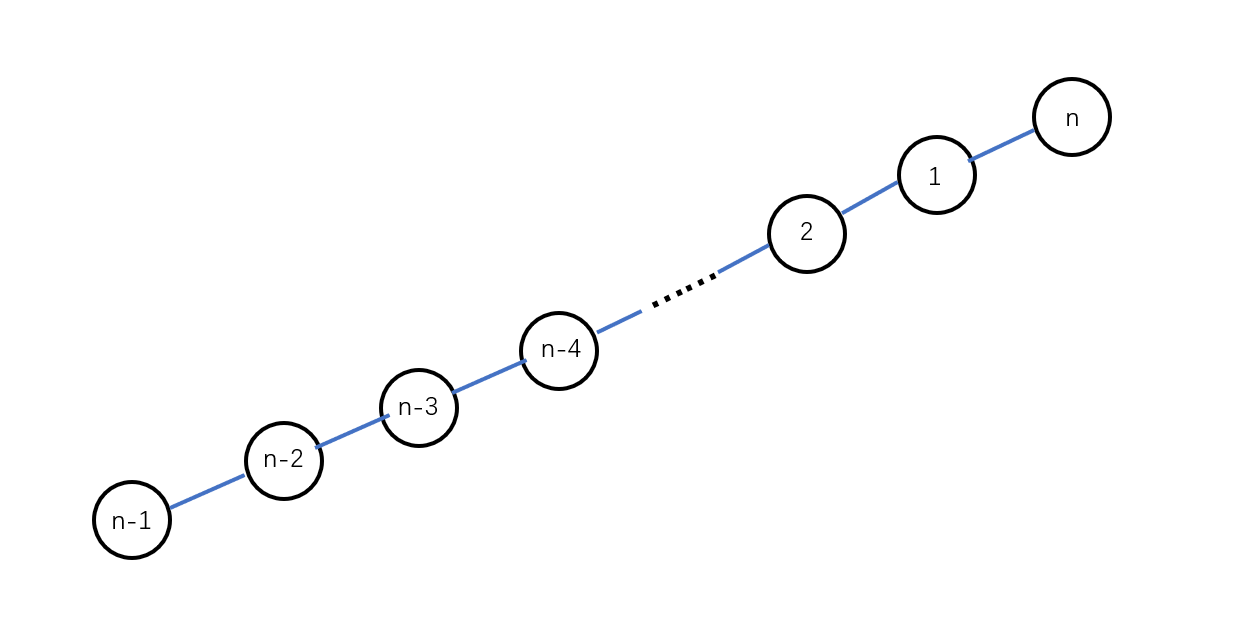
\includegraphics[scale=0.4]{figures/15_5.png}
\caption{ }
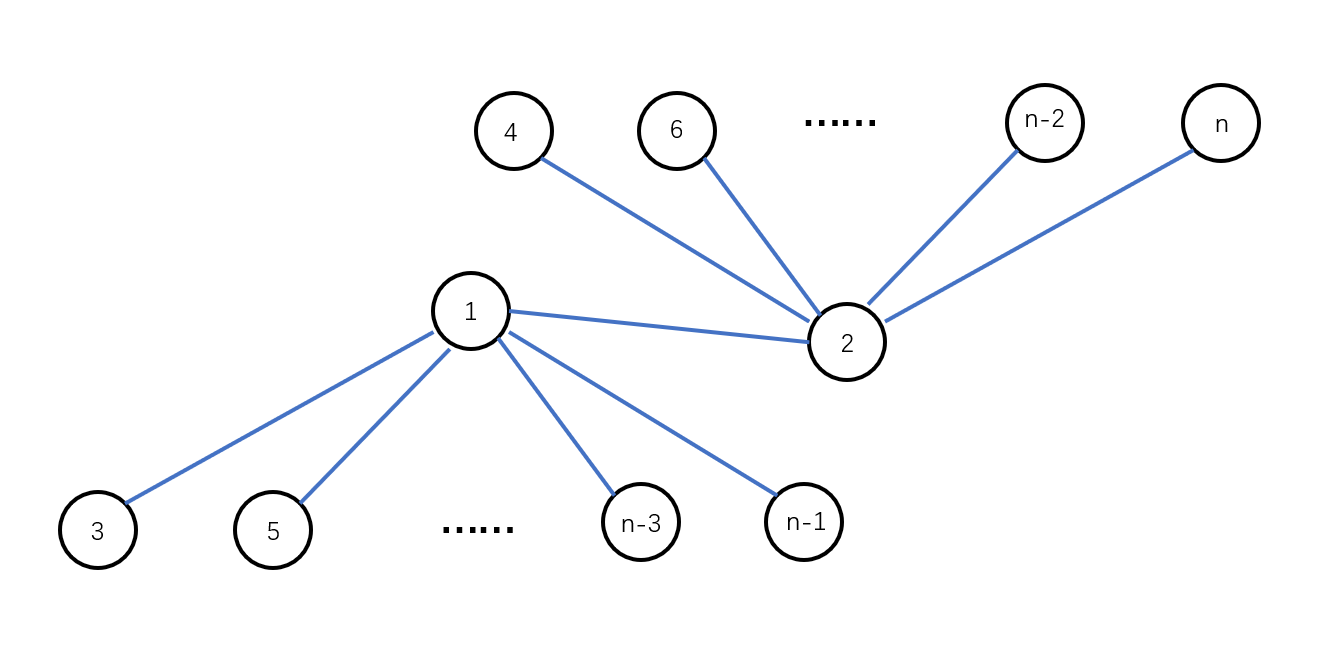
\includegraphics[scale=0.4]{figures/15_6.png}
\end{center}
\end{figure}
\begin{proof}
According to the algorithm to generate Pr\"ufer code:\\
1. Figure1: Cut the leaf 2,3,4\dots n-1 in turn, and so it's Pr\"ufer code is $(1,1,\dots,1)$.\\
2. Figure2: Cut the leaf n-1,1,2,3,4\dots n-3 in turn, and so it's Pr\"ufer code is $(1,2,3,\dots, n-2)$.\\
3. Figure3: Cut the leaf 1,2,3\dots n-2 in turn, and so it's Pr\"ufer code is $(3,4,5,\dots, n)$.\\
4. Figure4: Cut the leaf 1,2,n-1,n-2,n-3,\dots 4 in turn, and so it's Pr\"ufer code is $(n, n-1, n-2,\dots,4,3)$.\\
5. Figure5: Cut the leaf n-1,n-2,n-3,\dots 2 in turn, and so it's Pr\"ufer code is $(n-2,n-3,\dots,2,1)$.\\
6. Figure6: Cut the leaf 3,4,5,\dots ,n-1,1 in turn, and so it's Pr\"ufer code is $(1,2,1,2,\dots,1,2)$.\\
\end{proof}

The next two exercises use a bit of probability theory. Suppose we want to sample a random
tree on $[n]$. That is, we want to write a little procedure (say in Java) that uses randomness and outputs
a tree $T$ on $[n]$, where each of the $n^{n-2}$ trees has the same probability of 
appearing. 

\begin{exercise}
   Sketch how one could write such a procedure. Don't actually write program code, just
   describe it informally. You can assume you have access to a random generator
   \texttt{randomInt($n$)} that returns a function in $\{1,\dots,n\}$ as well
   as \texttt{randomReal()} that returns a random real number from the interval $[0,1]$.
\end{exercise}

Clearly, a tree $T$ on $[n]$ has at least $2$ and at most $n-1$ leaves. But how 
many leaves does it have on average? For this, we could use your tree sampler from the previous
exercise, run it 1000 times and compute the average. However, it would be much nicer to have 
a closed formula.

\begin{exercise}
  Fix some vertex $u \in [n]$. If we choose a tree $T$ on $[n]$ uniformly at random,
  what is the probability that $u$ is a leaf?
   What is the expected number of leaves of $T$?
\end{exercise}

\begin{exercise}
  For a fixed vertex $u$, what is the probability that $u$ has degree $2$?
\end{exercise}



\end{document}
